\section{Software Implementation}
The software part consists of two programs. The first one runs on Pico and is responsible for receiving commands from the PC, controlling the motor, acquiring data from the \gls{lidar} and sending the data back to the PC.
The second program runs on the PC and is responsible for determining the scanning density, receiving data from the Pico, parsing and processing the data, visualisation and storing of the point cloud.
\subsection{Pico program}
The Raspberry Pi Pico 2 W is programmed in Micropython. At the start of the program, the hardware is initialised and a Wi-Fi access point is created for the PC to connect to. 
After the connection is established, Pico waits for the PC to send the scanning density configuration, which is used to calculate the number of motor steps per scan. 

Before the scanning starts, the platform is rotated until the reference position is detected by the Hall effect sensor.
Then the main loop of the program starts. Each loop iteration is triggered by a command from the PC.
When the Pico receives the \texttt{r} command, it starts acquiring data from the \gls{lidar} for \SI{200}{\milli\second} and after that parses each valid \gls{lidar} packet, storing only the necessary information needed for reconstructing the point cloud. 
After that it sends the data to the PC with a \texttt{done} signal to indicate the end of the scan, and moves the platform to the next position.

Below is the pseudocode:
\begin{algorithm}[H]
\caption{Pico program}
\label{alg:pico-program}
\begin{algorithmic}

\State Initialise hardware
\State Initialise Wi-Fi access point
\State Wait for PC connection

\State Receive scan configuration from PC
\State Calculate number of motor steps per scan
\State Send ACK to PC

\State Perform platform homing

\While{program is running}

    \State Wait for command from PC

    \If{command is \texttt{r}}

        \State Mark start time

        \While{elapsed time is less than acquisition threshold}
            \State Read data from LiDAR UART
            \State Parse valid LiDAR packets
            \State Send compact packets to PC
        \EndWhile

        \State Send \texttt{done} to PC
        \State Move platform to next position

    \ElsIf{command is \texttt{stop}}

        \State Stop motor
        \State Send \texttt{restarting} to PC
        \State Restart program

    \EndIf
\EndWhile

\end{algorithmic}
\end{algorithm}

\subsection{PC program}
The PC program is written in Python. Since our application is mostly IO-bound, it is divided into two threads.

The receiver thread is responsible for communication with the Pico. It sends the trigger command to the Pico, receives the data, parses it and performs the necessary transformations to obtain the point cloud. It also computes the current azimuth angle of the platform based on the number of requests already sent to the Pico (platform makes a step after every request) and the scanning density.
The obtained points are then put into a global queue.

The main thread is responsible for visualisation. It creates an Open3D visualisation window and constantly checks the global queue for new data.
If there are new points, it updates the visualisation with the new data. Such separation allows the visualisation window to be responsive to user input even while the data is being received and processed in the background.

Below are the pseudocodes for both threads:
\begin{algorithm}[H]
\caption{PC main thread}
\label{alg:pc-main-thread}
\begin{algorithmic}
    \State Connect to Pico via Wi-Fi
    \State Send the scanning density config (\# of steps/scan) and wait for ACK
    \State Start receiver thread
    \State Initialise visualisation window
    \State Initialise Open3D point cloud containers for visualisation and export
    \While{acquisition is running}
        \State Read all available data from the global queue into a local container
        \If{local container is not empty}
            \State Update visualisation with the new dataf
            \If{\# of points in visualisation container > threshold}
                \State downsample visualisation container
            \EndIf
        \EndIf
        \State Update visualisation window with the current visualisation container
    \EndWhile
    \State Stop receiver thread
    \State Send \texttt{stop} command to Pico and wait for \texttt{restarting} message as an ACK
    \State Save export container on a machine
    \State Destroy visualisation window
\end{algorithmic}
\end{algorithm}
\begin{algorithm}[H]
\caption{PC receiver thread}
\label{alg:pc-receiver-thread}
\begin{algorithmic}
    \For{each platform position}
    \State Compute current azimuth angle
    \State Send trigger command to Pico \texttt{r}
    \Repeat
    \State Receive data chunk from Pico
    \State Append data chunk to a receive buffer
    \Until{\texttt{done} signal received}
    \State Parse data
    \State Perform transformation on the data (Polar -> Cartesian; 2D to 3D via platform tilt angle and azimuth angle)
    \State Put obtained points into a global queue
    \EndFor
\end{algorithmic}
\end{algorithm}

\subsection{Point cloud reconstruction}
\label{subsec:point_cloud_reconstruction}
The data received from the Pico is a stream of trimmed \gls{lidar} packets, containing only the start and stop angles and twelve distance measurements "sandwiched" between them.
The angle corresponding to each distance measurement is obtained by linear interpolation between the start and stop angles\footnote{\SI{360}{\degree} is added to the stop angle in a case where the stop angle is less than the start angle due to the wrap-around occurring between \SI{359}{\degree} and \SI{0}{\degree}}.
Then, the obtained polar coordinates are transformed into Cartesian coordinates in a 2D plane:
\begin{equation}
    x = r \cdot \cos(\alpha), \quad y = r \cdot \sin(\alpha), \quad z = 0,
\end{equation}
where $r$ is the distance measurement and $\alpha$ is the corresponding linearly interpolated angle. Since our \gls{lidar} performs only 2D scanning, all points initially lie in the xy-plane ($z=0$).

The obtained points are then transformed according to the current orientation of the \gls{lidar}. First, the points which are lying in xy-plane are rotated around x-axis by the angle $\phi$, corresponding to the platform tilt angle (hard-coded constant in PC program):
\begin{equation}
\begin{bmatrix}
    x_{\text{t}} \\
    y_{\text{t}} \\
    z_{\text{t}} \\
\end{bmatrix}
=
\begin{bmatrix}
    1 & 0 & 0 \\
    0 & \cos \phi & -\sin \phi \\
    0 & \sin \phi & \cos \phi \\
\end{bmatrix}
\begin{bmatrix}
    x \\
    y \\
    z \\
\end{bmatrix}.
\end{equation}
\begin{figure}[H]
    \centering
    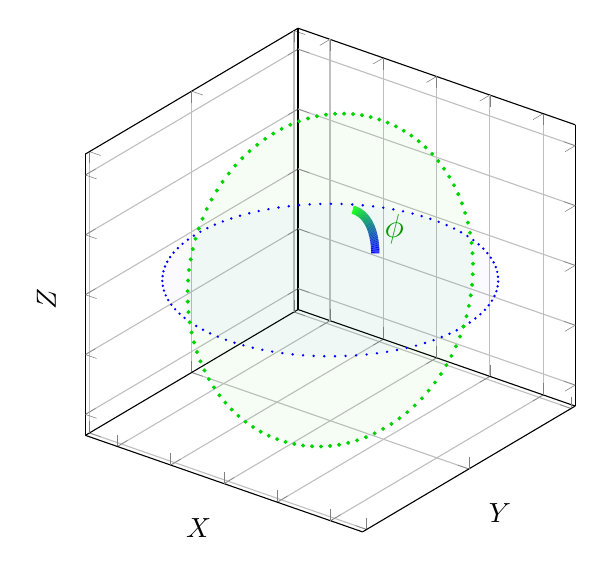
\begin{tikzpicture}
\begin{axis}[
    width=12cm,
    height=9cm,
    view={37.5}{27},
    axis equal image,
    scale only axis,
    grid=major,
    xlabel={$X$},
    ylabel={$Y$},
    zlabel={$Z$},
    xticklabels={},
    yticklabels={},
    zticklabels={},
    xmin=-5.2, xmax=5.2,
    ymin=-5.2, ymax=5.2,
    zmin=-4.7, zmax=4.7,
]
\addplot3[draw=none, fill=blue, fill opacity=0.02] coordinates {
(5.000000,0.000000,0.000000)
(4.989933,0.317120,0.000000)
(4.959774,0.632962,0.000000)
(4.909643,0.946256,0.000000)
(4.839744,1.255740,0.000000)
(4.750356,1.560167,0.000000)
(4.641840,1.858312,0.000000)
(4.514633,2.148975,0.000000)
(4.369247,2.430984,0.000000)
(4.206268,2.703204,0.000000)
(4.026351,2.964540,0.000000)
(3.830222,3.213938,0.000000)
(3.618670,3.450395,0.000000)
(3.392547,3.672959,0.000000)
(3.152763,3.880732,0.000000)
(2.900285,4.072880,0.000000)
(2.636127,4.248627,0.000000)
(2.361355,4.407267,0.000000)
(2.077075,4.548160,0.000000)
(1.784431,4.670739,0.000000)
(1.484602,4.774511,0.000000)
(1.178795,4.859058,0.000000)
(0.868241,4.924039,0.000000)
(0.554191,4.969192,0.000000)
(0.237910,4.994337,0.000000)
(-0.079330,4.999371,0.000000)
(-0.396250,4.984274,0.000000)
(-0.711574,4.949107,0.000000)
(-1.024033,4.894012,0.000000)
(-1.332369,4.819211,0.000000)
(-1.635340,4.725004,0.000000)
(-1.931726,4.611771,0.000000)
(-2.220333,4.479969,0.000000)
(-2.500000,4.330127,0.000000)
(-2.769600,4.162849,0.000000)
(-3.028048,3.978809,0.000000)
(-3.274304,3.778748,0.000000)
(-3.507374,3.563471,0.000000)
(-3.726322,3.333845,0.000000)
(-3.930265,3.090795,0.000000)
(-4.118383,2.835299,0.000000)
(-4.289917,2.568387,0.000000)
(-4.444177,2.291133,0.000000)
(-4.580542,2.004653,0.000000)
(-4.698463,1.710101,0.000000)
(-4.797465,1.408663,0.000000)
(-4.877149,1.101553,0.000000)
(-4.937194,0.790007,0.000000)
(-4.977360,0.475280,0.000000)
(-4.997483,0.158640,0.000000)
(-4.997483,-0.158640,0.000000)
(-4.977360,-0.475280,0.000000)
(-4.937194,-0.790007,0.000000)
(-4.877149,-1.101553,0.000000)
(-4.797465,-1.408663,0.000000)
(-4.698463,-1.710101,0.000000)
(-4.580542,-2.004653,0.000000)
(-4.444177,-2.291133,0.000000)
(-4.289917,-2.568387,0.000000)
(-4.118383,-2.835299,0.000000)
(-3.930265,-3.090795,0.000000)
(-3.726322,-3.333845,0.000000)
(-3.507374,-3.563471,0.000000)
(-3.274304,-3.778748,0.000000)
(-3.028048,-3.978809,0.000000)
(-2.769600,-4.162849,0.000000)
(-2.500000,-4.330127,0.000000)
(-2.220333,-4.479969,0.000000)
(-1.931726,-4.611771,0.000000)
(-1.635340,-4.725004,0.000000)
(-1.332369,-4.819211,0.000000)
(-1.024033,-4.894012,0.000000)
(-0.711574,-4.949107,0.000000)
(-0.396250,-4.984274,0.000000)
(-0.079330,-4.999371,0.000000)
(0.237910,-4.994337,0.000000)
(0.554191,-4.969192,0.000000)
(0.868241,-4.924039,0.000000)
(1.178795,-4.859058,0.000000)
(1.484602,-4.774511,0.000000)
(1.784431,-4.670739,0.000000)
(2.077075,-4.548160,0.000000)
(2.361355,-4.407267,0.000000)
(2.636127,-4.248627,0.000000)
(2.900285,-4.072880,0.000000)
(3.152763,-3.880732,0.000000)
(3.392547,-3.672959,0.000000)
(3.618670,-3.450395,0.000000)
(3.830222,-3.213938,0.000000)
(4.026351,-2.964540,0.000000)
(4.206268,-2.703204,0.000000)
(4.369247,-2.430984,0.000000)
(4.514633,-2.148975,0.000000)
(4.641840,-1.858312,0.000000)
(4.750356,-1.560167,0.000000)
(4.839744,-1.255740,0.000000)
(4.909643,-0.946256,0.000000)
(4.959774,-0.632962,0.000000)
(4.989933,-0.317120,0.000000)
(5.000000,-0.000000,0.000000)
} -- cycle;
\addplot3[draw=none, fill=green!80!black, fill opacity=0.04] coordinates {
(5.000000,0.000000,0.000000)
(4.989933,0.158560,0.274634)
(4.959774,0.316481,0.548161)
(4.909643,0.473128,0.819482)
(4.839744,0.627870,1.087503)
(4.750356,0.780084,1.351144)
(4.641840,0.929156,1.609346)
(4.514633,1.074487,1.861067)
(4.369247,1.215492,2.105294)
(4.206268,1.351602,2.341043)
(4.026351,1.482270,2.567367)
(3.830222,1.606969,2.783352)
(3.618670,1.725198,2.988130)
(3.392547,1.836479,3.180875)
(3.152763,1.940366,3.360813)
(2.900285,2.036440,3.527217)
(2.636127,2.124314,3.679419)
(2.361355,2.203633,3.816805)
(2.077075,2.274080,3.938822)
(1.784431,2.335370,4.044979)
(1.484602,2.387256,4.134848)
(1.178795,2.429529,4.208068)
(0.868241,2.462019,4.264343)
(0.554191,2.484596,4.303447)
(0.237910,2.497168,4.325222)
(-0.079330,2.499685,4.329582)
(-0.396250,2.492137,4.316508)
(-0.711574,2.474554,4.286053)
(-1.024033,2.447006,4.238339)
(-1.332369,2.409605,4.173559)
(-1.635340,2.362502,4.091974)
(-1.931726,2.305886,3.993911)
(-2.220333,2.239984,3.879767)
(-2.500000,2.165064,3.750000)
(-2.769600,2.081425,3.605133)
(-3.028048,1.989405,3.445750)
(-3.274304,1.889374,3.272492)
(-3.507374,1.781735,3.086056)
(-3.726322,1.666923,2.887194)
(-3.930265,1.545397,2.676707)
(-4.118383,1.417650,2.455441)
(-4.289917,1.284193,2.224288)
(-4.444177,1.145566,1.984179)
(-4.580542,1.002326,1.736080)
(-4.698463,0.855050,1.480991)
(-4.797465,0.704331,1.219938)
(-4.877149,0.550776,0.953973)
(-4.937194,0.395003,0.684166)
(-4.977360,0.237640,0.411605)
(-4.997483,0.079320,0.137386)
(-4.997483,-0.079320,-0.137386)
(-4.977360,-0.237640,-0.411605)
(-4.937194,-0.395003,-0.684166)
(-4.877149,-0.550776,-0.953973)
(-4.797465,-0.704331,-1.219938)
(-4.698463,-0.855050,-1.480991)
(-4.580542,-1.002326,-1.736080)
(-4.444177,-1.145566,-1.984179)
(-4.289917,-1.284193,-2.224288)
(-4.118383,-1.417650,-2.455441)
(-3.930265,-1.545397,-2.676707)
(-3.726322,-1.666923,-2.887194)
(-3.507374,-1.781735,-3.086056)
(-3.274304,-1.889374,-3.272492)
(-3.028048,-1.989405,-3.445750)
(-2.769600,-2.081425,-3.605133)
(-2.500000,-2.165064,-3.750000)
(-2.220333,-2.239984,-3.879767)
(-1.931726,-2.305886,-3.993911)
(-1.635340,-2.362502,-4.091974)
(-1.332369,-2.409605,-4.173559)
(-1.024033,-2.447006,-4.238339)
(-0.711574,-2.474554,-4.286053)
(-0.396250,-2.492137,-4.316508)
(-0.079330,-2.499685,-4.329582)
(0.237910,-2.497168,-4.325222)
(0.554191,-2.484596,-4.303447)
(0.868241,-2.462019,-4.264343)
(1.178795,-2.429529,-4.208068)
(1.484602,-2.387256,-4.134848)
(1.784431,-2.335370,-4.044979)
(2.077075,-2.274080,-3.938822)
(2.361355,-2.203633,-3.816805)
(2.636127,-2.124314,-3.679419)
(2.900285,-2.036440,-3.527217)
(3.152763,-1.940366,-3.360813)
(3.392547,-1.836479,-3.180875)
(3.618670,-1.725198,-2.988130)
(3.830222,-1.606969,-2.783352)
(4.026351,-1.482270,-2.567367)
(4.206268,-1.351602,-2.341043)
(4.369247,-1.215492,-2.105294)
(4.514633,-1.074487,-1.861067)
(4.641840,-0.929156,-1.609346)
(4.750356,-0.780084,-1.351144)
(4.839744,-0.627870,-1.087503)
(4.909643,-0.473128,-0.819482)
(4.959774,-0.316481,-0.548161)
(4.989933,-0.158560,-0.274634)
(5.000000,-0.000000,-0.000000)
} -- cycle;
\addplot3[only marks, mark=*, mark size=0.20pt, blue] coordinates {
(5.000000,0.000000,0.000000)
(4.989933,0.317120,0.000000)
(4.959774,0.632962,0.000000)
(4.909643,0.946256,0.000000)
(4.839744,1.255740,0.000000)
(4.750356,1.560167,0.000000)
(4.641840,1.858312,0.000000)
(4.514633,2.148975,0.000000)
(4.369247,2.430984,0.000000)
(4.206268,2.703204,0.000000)
(4.026351,2.964540,0.000000)
(3.830222,3.213938,0.000000)
(3.618670,3.450395,0.000000)
(3.392547,3.672959,0.000000)
(3.152763,3.880732,0.000000)
(2.900285,4.072880,0.000000)
(2.636127,4.248627,0.000000)
(2.361355,4.407267,0.000000)
(2.077075,4.548160,0.000000)
(1.784431,4.670739,0.000000)
(1.484602,4.774511,0.000000)
(1.178795,4.859058,0.000000)
(0.868241,4.924039,0.000000)
(0.554191,4.969192,0.000000)
(0.237910,4.994337,0.000000)
(-0.079330,4.999371,0.000000)
(-0.396250,4.984274,0.000000)
(-0.711574,4.949107,0.000000)
(-1.024033,4.894012,0.000000)
(-1.332369,4.819211,0.000000)
(-1.635340,4.725004,0.000000)
(-1.931726,4.611771,0.000000)
(-2.220333,4.479969,0.000000)
(-2.500000,4.330127,0.000000)
(-2.769600,4.162849,0.000000)
(-3.028048,3.978809,0.000000)
(-3.274304,3.778748,0.000000)
(-3.507374,3.563471,0.000000)
(-3.726322,3.333845,0.000000)
(-3.930265,3.090795,0.000000)
(-4.118383,2.835299,0.000000)
(-4.289917,2.568387,0.000000)
(-4.444177,2.291133,0.000000)
(-4.580542,2.004653,0.000000)
(-4.698463,1.710101,0.000000)
(-4.797465,1.408663,0.000000)
(-4.877149,1.101553,0.000000)
(-4.937194,0.790007,0.000000)
(-4.977360,0.475280,0.000000)
(-4.997483,0.158640,0.000000)
(-4.997483,-0.158640,0.000000)
(-4.977360,-0.475280,0.000000)
(-4.937194,-0.790007,0.000000)
(-4.877149,-1.101553,0.000000)
(-4.797465,-1.408663,0.000000)
(-4.698463,-1.710101,0.000000)
(-4.580542,-2.004653,0.000000)
(-4.444177,-2.291133,0.000000)
(-4.289917,-2.568387,0.000000)
(-4.118383,-2.835299,0.000000)
(-3.930265,-3.090795,0.000000)
(-3.726322,-3.333845,0.000000)
(-3.507374,-3.563471,0.000000)
(-3.274304,-3.778748,0.000000)
(-3.028048,-3.978809,0.000000)
(-2.769600,-4.162849,0.000000)
(-2.500000,-4.330127,0.000000)
(-2.220333,-4.479969,0.000000)
(-1.931726,-4.611771,0.000000)
(-1.635340,-4.725004,0.000000)
(-1.332369,-4.819211,0.000000)
(-1.024033,-4.894012,0.000000)
(-0.711574,-4.949107,0.000000)
(-0.396250,-4.984274,0.000000)
(-0.079330,-4.999371,0.000000)
(0.237910,-4.994337,0.000000)
(0.554191,-4.969192,0.000000)
(0.868241,-4.924039,0.000000)
(1.178795,-4.859058,0.000000)
(1.484602,-4.774511,0.000000)
(1.784431,-4.670739,0.000000)
(2.077075,-4.548160,0.000000)
(2.361355,-4.407267,0.000000)
(2.636127,-4.248627,0.000000)
(2.900285,-4.072880,0.000000)
(3.152763,-3.880732,0.000000)
(3.392547,-3.672959,0.000000)
(3.618670,-3.450395,0.000000)
(3.830222,-3.213938,0.000000)
(4.026351,-2.964540,0.000000)
(4.206268,-2.703204,0.000000)
(4.369247,-2.430984,0.000000)
(4.514633,-2.148975,0.000000)
(4.641840,-1.858312,0.000000)
(4.750356,-1.560167,0.000000)
(4.839744,-1.255740,0.000000)
(4.909643,-0.946256,0.000000)
(4.959774,-0.632962,0.000000)
(4.989933,-0.317120,0.000000)
(5.000000,-0.000000,0.000000)
};
\addplot3[only marks, mark=*, mark size=0.50pt, green!83!black] coordinates {
(5.000000,0.000000,0.000000)
(4.989933,0.158560,0.274634)
(4.959774,0.316481,0.548161)
(4.909643,0.473128,0.819482)
(4.839744,0.627870,1.087503)
(4.750356,0.780084,1.351144)
(4.641840,0.929156,1.609346)
(4.514633,1.074487,1.861067)
(4.369247,1.215492,2.105294)
(4.206268,1.351602,2.341043)
(4.026351,1.482270,2.567367)
(3.830222,1.606969,2.783352)
(3.618670,1.725198,2.988130)
(3.392547,1.836479,3.180875)
(3.152763,1.940366,3.360813)
(2.900285,2.036440,3.527217)
(2.636127,2.124314,3.679419)
(2.361355,2.203633,3.816805)
(2.077075,2.274080,3.938822)
(1.784431,2.335370,4.044979)
(1.484602,2.387256,4.134848)
(1.178795,2.429529,4.208068)
(0.868241,2.462019,4.264343)
(0.554191,2.484596,4.303447)
(0.237910,2.497168,4.325222)
(-0.079330,2.499685,4.329582)
(-0.396250,2.492137,4.316508)
(-0.711574,2.474554,4.286053)
(-1.024033,2.447006,4.238339)
(-1.332369,2.409605,4.173559)
(-1.635340,2.362502,4.091974)
(-1.931726,2.305886,3.993911)
(-2.220333,2.239984,3.879767)
(-2.500000,2.165064,3.750000)
(-2.769600,2.081425,3.605133)
(-3.028048,1.989405,3.445750)
(-3.274304,1.889374,3.272492)
(-3.507374,1.781735,3.086056)
(-3.726322,1.666923,2.887194)
(-3.930265,1.545397,2.676707)
(-4.118383,1.417650,2.455441)
(-4.289917,1.284193,2.224288)
(-4.444177,1.145566,1.984179)
(-4.580542,1.002326,1.736080)
(-4.698463,0.855050,1.480991)
(-4.797465,0.704331,1.219938)
(-4.877149,0.550776,0.953973)
(-4.937194,0.395003,0.684166)
(-4.977360,0.237640,0.411605)
(-4.997483,0.079320,0.137386)
(-4.997483,-0.079320,-0.137386)
(-4.977360,-0.237640,-0.411605)
(-4.937194,-0.395003,-0.684166)
(-4.877149,-0.550776,-0.953973)
(-4.797465,-0.704331,-1.219938)
(-4.698463,-0.855050,-1.480991)
(-4.580542,-1.002326,-1.736080)
(-4.444177,-1.145566,-1.984179)
(-4.289917,-1.284193,-2.224288)
(-4.118383,-1.417650,-2.455441)
(-3.930265,-1.545397,-2.676707)
(-3.726322,-1.666923,-2.887194)
(-3.507374,-1.781735,-3.086056)
(-3.274304,-1.889374,-3.272492)
(-3.028048,-1.989405,-3.445750)
(-2.769600,-2.081425,-3.605133)
(-2.500000,-2.165064,-3.750000)
(-2.220333,-2.239984,-3.879767)
(-1.931726,-2.305886,-3.993911)
(-1.635340,-2.362502,-4.091974)
(-1.332369,-2.409605,-4.173559)
(-1.024033,-2.447006,-4.238339)
(-0.711574,-2.474554,-4.286053)
(-0.396250,-2.492137,-4.316508)
(-0.079330,-2.499685,-4.329582)
(0.237910,-2.497168,-4.325222)
(0.554191,-2.484596,-4.303447)
(0.868241,-2.462019,-4.264343)
(1.178795,-2.429529,-4.208068)
(1.484602,-2.387256,-4.134848)
(1.784431,-2.335370,-4.044979)
(2.077075,-2.274080,-3.938822)
(2.361355,-2.203633,-3.816805)
(2.636127,-2.124314,-3.679419)
(2.900285,-2.036440,-3.527217)
(3.152763,-1.940366,-3.360813)
(3.392547,-1.836479,-3.180875)
(3.618670,-1.725198,-2.988130)
(3.830222,-1.606969,-2.783352)
(4.026351,-1.482270,-2.567367)
(4.206268,-1.351602,-2.341043)
(4.369247,-1.215492,-2.105294)
(4.514633,-1.074487,-1.861067)
(4.641840,-0.929156,-1.609346)
(4.750356,-0.780084,-1.351144)
(4.839744,-0.627870,-1.087503)
(4.909643,-0.473128,-0.819482)
(4.959774,-0.316481,-0.548161)
(4.989933,-0.158560,-0.274634)
(5.000000,-0.000000,-0.000000)
};
\addplot3[color={rgb,1:red,0.0000;green,0.0000;blue,1.0000}, line width=3pt] coordinates {(0.000000,2.200000,0.000000) (0.000000,2.199877,0.023271)};
\addplot3[color={rgb,1:red,0.0000;green,0.0102;blue,0.9898}, line width=3pt] coordinates {(0.000000,2.199877,0.023271) (0.000000,2.199508,0.046539)};
\addplot3[color={rgb,1:red,0.0000;green,0.0204;blue,0.9796}, line width=3pt] coordinates {(0.000000,2.199508,0.046539) (0.000000,2.198892,0.069801)};
\addplot3[color={rgb,1:red,0.0000;green,0.0306;blue,0.9694}, line width=3pt] coordinates {(0.000000,2.198892,0.069801) (0.000000,2.198031,0.093056)};
\addplot3[color={rgb,1:red,0.0000;green,0.0408;blue,0.9592}, line width=3pt] coordinates {(0.000000,2.198031,0.093056) (0.000000,2.196924,0.116301)};
\addplot3[color={rgb,1:red,0.0000;green,0.0510;blue,0.9490}, line width=3pt] coordinates {(0.000000,2.196924,0.116301) (0.000000,2.195571,0.139533)};
\addplot3[color={rgb,1:red,0.0000;green,0.0612;blue,0.9388}, line width=3pt] coordinates {(0.000000,2.195571,0.139533) (0.000000,2.193972,0.162749)};
\addplot3[color={rgb,1:red,0.0000;green,0.0714;blue,0.9286}, line width=3pt] coordinates {(0.000000,2.193972,0.162749) (0.000000,2.192128,0.185946)};
\addplot3[color={rgb,1:red,0.0000;green,0.0816;blue,0.9184}, line width=3pt] coordinates {(0.000000,2.192128,0.185946) (0.000000,2.190038,0.209123)};
\addplot3[color={rgb,1:red,0.0000;green,0.0918;blue,0.9082}, line width=3pt] coordinates {(0.000000,2.190038,0.209123) (0.000000,2.187704,0.232277)};
\addplot3[color={rgb,1:red,0.0000;green,0.1020;blue,0.8980}, line width=3pt] coordinates {(0.000000,2.187704,0.232277) (0.000000,2.185124,0.255404)};
\addplot3[color={rgb,1:red,0.0000;green,0.1122;blue,0.8878}, line width=3pt] coordinates {(0.000000,2.185124,0.255404) (0.000000,2.182301,0.278503)};
\addplot3[color={rgb,1:red,0.0000;green,0.1224;blue,0.8776}, line width=3pt] coordinates {(0.000000,2.182301,0.278503) (0.000000,2.179233,0.301571)};
\addplot3[color={rgb,1:red,0.0000;green,0.1327;blue,0.8673}, line width=3pt] coordinates {(0.000000,2.179233,0.301571) (0.000000,2.175921,0.324605)};
\addplot3[color={rgb,1:red,0.0000;green,0.1429;blue,0.8571}, line width=3pt] coordinates {(0.000000,2.175921,0.324605) (0.000000,2.172366,0.347603)};
\addplot3[color={rgb,1:red,0.0000;green,0.1531;blue,0.8469}, line width=3pt] coordinates {(0.000000,2.172366,0.347603) (0.000000,2.168567,0.370562)};
\addplot3[color={rgb,1:red,0.0000;green,0.1633;blue,0.8367}, line width=3pt] coordinates {(0.000000,2.168567,0.370562) (0.000000,2.164526,0.393479)};
\addplot3[color={rgb,1:red,0.0000;green,0.1735;blue,0.8265}, line width=3pt] coordinates {(0.000000,2.164526,0.393479) (0.000000,2.160243,0.416353)};
\addplot3[color={rgb,1:red,0.0000;green,0.1837;blue,0.8163}, line width=3pt] coordinates {(0.000000,2.160243,0.416353) (0.000000,2.155718,0.439180)};
\addplot3[color={rgb,1:red,0.0000;green,0.1939;blue,0.8061}, line width=3pt] coordinates {(0.000000,2.155718,0.439180) (0.000000,2.150952,0.461957)};
\addplot3[color={rgb,1:red,0.0000;green,0.2041;blue,0.7959}, line width=3pt] coordinates {(0.000000,2.150952,0.461957) (0.000000,2.145946,0.484683)};
\addplot3[color={rgb,1:red,0.0000;green,0.2143;blue,0.7857}, line width=3pt] coordinates {(0.000000,2.145946,0.484683) (0.000000,2.140699,0.507355)};
\addplot3[color={rgb,1:red,0.0000;green,0.2245;blue,0.7755}, line width=3pt] coordinates {(0.000000,2.140699,0.507355) (0.000000,2.135212,0.529970)};
\addplot3[color={rgb,1:red,0.0000;green,0.2347;blue,0.7653}, line width=3pt] coordinates {(0.000000,2.135212,0.529970) (0.000000,2.129487,0.552526)};
\addplot3[color={rgb,1:red,0.0000;green,0.2449;blue,0.7551}, line width=3pt] coordinates {(0.000000,2.129487,0.552526) (0.000000,2.123524,0.575019)};
\addplot3[color={rgb,1:red,0.0000;green,0.2551;blue,0.7449}, line width=3pt] coordinates {(0.000000,2.123524,0.575019) (0.000000,2.117323,0.597449)};
\addplot3[color={rgb,1:red,0.0000;green,0.2653;blue,0.7347}, line width=3pt] coordinates {(0.000000,2.117323,0.597449) (0.000000,2.110885,0.619812)};
\addplot3[color={rgb,1:red,0.0000;green,0.2755;blue,0.7245}, line width=3pt] coordinates {(0.000000,2.110885,0.619812) (0.000000,2.104210,0.642105)};
\addplot3[color={rgb,1:red,0.0000;green,0.2857;blue,0.7143}, line width=3pt] coordinates {(0.000000,2.104210,0.642105) (0.000000,2.097301,0.664326)};
\addplot3[color={rgb,1:red,0.0000;green,0.2959;blue,0.7041}, line width=3pt] coordinates {(0.000000,2.097301,0.664326) (0.000000,2.090156,0.686474)};
\addplot3[color={rgb,1:red,0.0000;green,0.3061;blue,0.6939}, line width=3pt] coordinates {(0.000000,2.090156,0.686474) (0.000000,2.082778,0.708544)};
\addplot3[color={rgb,1:red,0.0000;green,0.3163;blue,0.6837}, line width=3pt] coordinates {(0.000000,2.082778,0.708544) (0.000000,2.075167,0.730535)};
\addplot3[color={rgb,1:red,0.0000;green,0.3265;blue,0.6735}, line width=3pt] coordinates {(0.000000,2.075167,0.730535) (0.000000,2.067324,0.752444)};
\addplot3[color={rgb,1:red,0.0000;green,0.3367;blue,0.6633}, line width=3pt] coordinates {(0.000000,2.067324,0.752444) (0.000000,2.059249,0.774269)};
\addplot3[color={rgb,1:red,0.0000;green,0.3469;blue,0.6531}, line width=3pt] coordinates {(0.000000,2.059249,0.774269) (0.000000,2.050944,0.796008)};
\addplot3[color={rgb,1:red,0.0000;green,0.3571;blue,0.6429}, line width=3pt] coordinates {(0.000000,2.050944,0.796008) (0.000000,2.042409,0.817657)};
\addplot3[color={rgb,1:red,0.0000;green,0.3673;blue,0.6327}, line width=3pt] coordinates {(0.000000,2.042409,0.817657) (0.000000,2.033646,0.839215)};
\addplot3[color={rgb,1:red,0.0000;green,0.3776;blue,0.6224}, line width=3pt] coordinates {(0.000000,2.033646,0.839215) (0.000000,2.024656,0.860679)};
\addplot3[color={rgb,1:red,0.0000;green,0.3878;blue,0.6122}, line width=3pt] coordinates {(0.000000,2.024656,0.860679) (0.000000,2.015439,0.882047)};
\addplot3[color={rgb,1:red,0.0000;green,0.3980;blue,0.6020}, line width=3pt] coordinates {(0.000000,2.015439,0.882047) (0.000000,2.005996,0.903316)};
\addplot3[color={rgb,1:red,0.0000;green,0.4082;blue,0.5918}, line width=3pt] coordinates {(0.000000,2.005996,0.903316) (0.000000,1.996329,0.924484)};
\addplot3[color={rgb,1:red,0.0000;green,0.4184;blue,0.5816}, line width=3pt] coordinates {(0.000000,1.996329,0.924484) (0.000000,1.986438,0.945549)};
\addplot3[color={rgb,1:red,0.0000;green,0.4286;blue,0.5714}, line width=3pt] coordinates {(0.000000,1.986438,0.945549) (0.000000,1.976326,0.966508)};
\addplot3[color={rgb,1:red,0.0000;green,0.4388;blue,0.5612}, line width=3pt] coordinates {(0.000000,1.976326,0.966508) (0.000000,1.965992,0.987358)};
\addplot3[color={rgb,1:red,0.0000;green,0.4490;blue,0.5510}, line width=3pt] coordinates {(0.000000,1.965992,0.987358) (0.000000,1.955438,1.008098)};
\addplot3[color={rgb,1:red,0.0000;green,0.4592;blue,0.5408}, line width=3pt] coordinates {(0.000000,1.955438,1.008098) (0.000000,1.944665,1.028726)};
\addplot3[color={rgb,1:red,0.0000;green,0.4694;blue,0.5306}, line width=3pt] coordinates {(0.000000,1.944665,1.028726) (0.000000,1.933675,1.049238)};
\addplot3[color={rgb,1:red,0.0000;green,0.4796;blue,0.5204}, line width=3pt] coordinates {(0.000000,1.933675,1.049238) (0.000000,1.922469,1.069633)};
\addplot3[color={rgb,1:red,0.0000;green,0.4898;blue,0.5102}, line width=3pt] coordinates {(0.000000,1.922469,1.069633) (0.000000,1.911047,1.089908)};
\addplot3[color={rgb,1:red,0.0000;green,0.5000;blue,0.5000}, line width=3pt] coordinates {(0.000000,1.911047,1.089908) (0.000000,1.899412,1.110061)};
\addplot3[color={rgb,1:red,0.0000;green,0.5102;blue,0.4898}, line width=3pt] coordinates {(0.000000,1.899412,1.110061) (0.000000,1.887564,1.130090)};
\addplot3[color={rgb,1:red,0.0000;green,0.5204;blue,0.4796}, line width=3pt] coordinates {(0.000000,1.887564,1.130090) (0.000000,1.875504,1.149993)};
\addplot3[color={rgb,1:red,0.0000;green,0.5306;blue,0.4694}, line width=3pt] coordinates {(0.000000,1.875504,1.149993) (0.000000,1.863235,1.169767)};
\addplot3[color={rgb,1:red,0.0000;green,0.5408;blue,0.4592}, line width=3pt] coordinates {(0.000000,1.863235,1.169767) (0.000000,1.850758,1.189410)};
\addplot3[color={rgb,1:red,0.0000;green,0.5510;blue,0.4490}, line width=3pt] coordinates {(0.000000,1.850758,1.189410) (0.000000,1.838073,1.208920)};
\addplot3[color={rgb,1:red,0.0000;green,0.5612;blue,0.4388}, line width=3pt] coordinates {(0.000000,1.838073,1.208920) (0.000000,1.825183,1.228294)};
\addplot3[color={rgb,1:red,0.0000;green,0.5714;blue,0.4286}, line width=3pt] coordinates {(0.000000,1.825183,1.228294) (0.000000,1.812088,1.247532)};
\addplot3[color={rgb,1:red,0.0000;green,0.5816;blue,0.4184}, line width=3pt] coordinates {(0.000000,1.812088,1.247532) (0.000000,1.798791,1.266629)};
\addplot3[color={rgb,1:red,0.0000;green,0.5918;blue,0.4082}, line width=3pt] coordinates {(0.000000,1.798791,1.266629) (0.000000,1.785293,1.285585)};
\addplot3[color={rgb,1:red,0.0000;green,0.6020;blue,0.3980}, line width=3pt] coordinates {(0.000000,1.785293,1.285585) (0.000000,1.771595,1.304397)};
\addplot3[color={rgb,1:red,0.0000;green,0.6122;blue,0.3878}, line width=3pt] coordinates {(0.000000,1.771595,1.304397) (0.000000,1.757698,1.323064)};
\addplot3[color={rgb,1:red,0.0000;green,0.6224;blue,0.3776}, line width=3pt] coordinates {(0.000000,1.757698,1.323064) (0.000000,1.743605,1.341582)};
\addplot3[color={rgb,1:red,0.0000;green,0.6327;blue,0.3673}, line width=3pt] coordinates {(0.000000,1.743605,1.341582) (0.000000,1.729317,1.359950)};
\addplot3[color={rgb,1:red,0.0000;green,0.6429;blue,0.3571}, line width=3pt] coordinates {(0.000000,1.729317,1.359950) (0.000000,1.714835,1.378166)};
\addplot3[color={rgb,1:red,0.0000;green,0.6531;blue,0.3469}, line width=3pt] coordinates {(0.000000,1.714835,1.378166) (0.000000,1.700162,1.396227)};
\addplot3[color={rgb,1:red,0.0000;green,0.6633;blue,0.3367}, line width=3pt] coordinates {(0.000000,1.700162,1.396227) (0.000000,1.685298,1.414133)};
\addplot3[color={rgb,1:red,0.0000;green,0.6735;blue,0.3265}, line width=3pt] coordinates {(0.000000,1.685298,1.414133) (0.000000,1.670245,1.431880)};
\addplot3[color={rgb,1:red,0.0000;green,0.6837;blue,0.3163}, line width=3pt] coordinates {(0.000000,1.670245,1.431880) (0.000000,1.655006,1.449467)};
\addplot3[color={rgb,1:red,0.0000;green,0.6939;blue,0.3061}, line width=3pt] coordinates {(0.000000,1.655006,1.449467) (0.000000,1.639582,1.466892)};
\addplot3[color={rgb,1:red,0.0000;green,0.7041;blue,0.2959}, line width=3pt] coordinates {(0.000000,1.639582,1.466892) (0.000000,1.623974,1.484153)};
\addplot3[color={rgb,1:red,0.0000;green,0.7143;blue,0.2857}, line width=3pt] coordinates {(0.000000,1.623974,1.484153) (0.000000,1.608184,1.501247)};
\addplot3[color={rgb,1:red,0.0000;green,0.7245;blue,0.2755}, line width=3pt] coordinates {(0.000000,1.608184,1.501247) (0.000000,1.592215,1.518174)};
\addplot3[color={rgb,1:red,0.0000;green,0.7347;blue,0.2653}, line width=3pt] coordinates {(0.000000,1.592215,1.518174) (0.000000,1.576067,1.534931)};
\addplot3[color={rgb,1:red,0.0000;green,0.7449;blue,0.2551}, line width=3pt] coordinates {(0.000000,1.576067,1.534931) (0.000000,1.559743,1.551516)};
\addplot3[color={rgb,1:red,0.0000;green,0.7551;blue,0.2449}, line width=3pt] coordinates {(0.000000,1.559743,1.551516) (0.000000,1.543245,1.567927)};
\addplot3[color={rgb,1:red,0.0000;green,0.7653;blue,0.2347}, line width=3pt] coordinates {(0.000000,1.543245,1.567927) (0.000000,1.526574,1.584163)};
\addplot3[color={rgb,1:red,0.0000;green,0.7755;blue,0.2245}, line width=3pt] coordinates {(0.000000,1.526574,1.584163) (0.000000,1.509732,1.600222)};
\addplot3[color={rgb,1:red,0.0000;green,0.7857;blue,0.2143}, line width=3pt] coordinates {(0.000000,1.509732,1.600222) (0.000000,1.492721,1.616102)};
\addplot3[color={rgb,1:red,0.0000;green,0.7959;blue,0.2041}, line width=3pt] coordinates {(0.000000,1.492721,1.616102) (0.000000,1.475543,1.631801)};
\addplot3[color={rgb,1:red,0.0000;green,0.8061;blue,0.1939}, line width=3pt] coordinates {(0.000000,1.475543,1.631801) (0.000000,1.458200,1.647317)};
\addplot3[color={rgb,1:red,0.0000;green,0.8163;blue,0.1837}, line width=3pt] coordinates {(0.000000,1.458200,1.647317) (0.000000,1.440694,1.662649)};
\addplot3[color={rgb,1:red,0.0000;green,0.8265;blue,0.1735}, line width=3pt] coordinates {(0.000000,1.440694,1.662649) (0.000000,1.423026,1.677795)};
\addplot3[color={rgb,1:red,0.0000;green,0.8367;blue,0.1633}, line width=3pt] coordinates {(0.000000,1.423026,1.677795) (0.000000,1.405200,1.692753)};
\addplot3[color={rgb,1:red,0.0000;green,0.8469;blue,0.1531}, line width=3pt] coordinates {(0.000000,1.405200,1.692753) (0.000000,1.387216,1.707522)};
\addplot3[color={rgb,1:red,0.0000;green,0.8571;blue,0.1429}, line width=3pt] coordinates {(0.000000,1.387216,1.707522) (0.000000,1.369077,1.722100)};
\addplot3[color={rgb,1:red,0.0000;green,0.8673;blue,0.1327}, line width=3pt] coordinates {(0.000000,1.369077,1.722100) (0.000000,1.350785,1.736485)};
\addplot3[color={rgb,1:red,0.0000;green,0.8776;blue,0.1224}, line width=3pt] coordinates {(0.000000,1.350785,1.736485) (0.000000,1.332341,1.750676)};
\addplot3[color={rgb,1:red,0.0000;green,0.8878;blue,0.1122}, line width=3pt] coordinates {(0.000000,1.332341,1.750676) (0.000000,1.313749,1.764671)};
\addplot3[color={rgb,1:red,0.0000;green,0.8980;blue,0.1020}, line width=3pt] coordinates {(0.000000,1.313749,1.764671) (0.000000,1.295009,1.778469)};
\addplot3[color={rgb,1:red,0.0000;green,0.9082;blue,0.0918}, line width=3pt] coordinates {(0.000000,1.295009,1.778469) (0.000000,1.276125,1.792067)};
\addplot3[color={rgb,1:red,0.0000;green,0.9184;blue,0.0816}, line width=3pt] coordinates {(0.000000,1.276125,1.792067) (0.000000,1.257098,1.805465)};
\addplot3[color={rgb,1:red,0.0000;green,0.9286;blue,0.0714}, line width=3pt] coordinates {(0.000000,1.257098,1.805465) (0.000000,1.237930,1.818661)};
\addplot3[color={rgb,1:red,0.0000;green,0.9388;blue,0.0612}, line width=3pt] coordinates {(0.000000,1.237930,1.818661) (0.000000,1.218624,1.831654)};
\addplot3[color={rgb,1:red,0.0000;green,0.9490;blue,0.0510}, line width=3pt] coordinates {(0.000000,1.218624,1.831654) (0.000000,1.199182,1.844441)};
\addplot3[color={rgb,1:red,0.0000;green,0.9592;blue,0.0408}, line width=3pt] coordinates {(0.000000,1.199182,1.844441) (0.000000,1.179605,1.857022)};
\addplot3[color={rgb,1:red,0.0000;green,0.9694;blue,0.0306}, line width=3pt] coordinates {(0.000000,1.179605,1.857022) (0.000000,1.159896,1.869396)};
\addplot3[color={rgb,1:red,0.0000;green,0.9796;blue,0.0204}, line width=3pt] coordinates {(0.000000,1.159896,1.869396) (0.000000,1.140057,1.881560)};
\addplot3[color={rgb,1:red,0.0000;green,0.9898;blue,0.0102}, line width=3pt] coordinates {(0.000000,1.140057,1.881560) (0.000000,1.120091,1.893514)};
\addplot3[color={rgb,1:red,0.0000;green,1.0000;blue,0.0000}, line width=3pt] coordinates {(0.000000,1.120091,1.893514) (0.000000,1.100000,1.905256)};
\node[green!60!black, font=\large] at (axis cs:1.3,1.428942,1.525000) {$\phi$};
\end{axis}
\end{tikzpicture}

    \caption{Visualisation of the tilt transformation}
\end{figure}

After the tilt transformation, the points are rotated around the z-axis by the angle $\theta$, corresponding to the current platform azimuth:
\begin{equation}
\begin{bmatrix}
    x_{\text{a}} \\
    y_{\text{a}} \\
    z_{\text{a}} \\
\end{bmatrix}
=
\begin{bmatrix}
    \cos \theta & -\sin \theta & 0 \\
    \sin \theta & \cos \theta & 0 \\
    0 & 0 & 1 \\
\end{bmatrix}
\begin{bmatrix}
    x_{\text{t}} \\
    y_{\text{t}} \\
    z_{\text{t}} \\
\end{bmatrix}.
\end{equation}
\begin{figure}[H]
    \centering
    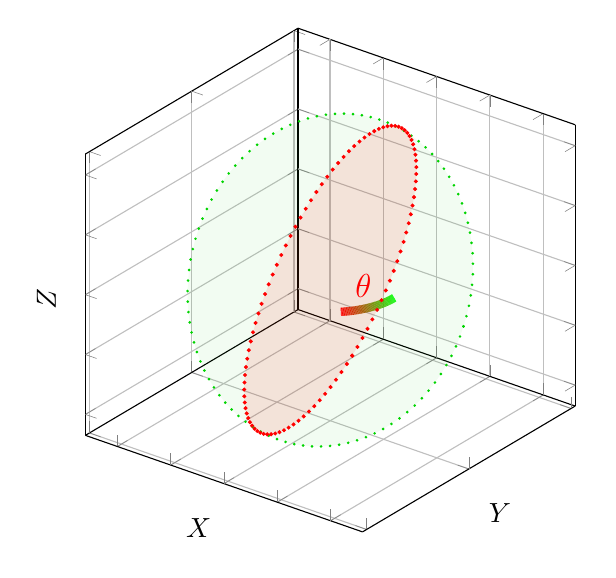
\begin{tikzpicture}
\begin{axis}[
    width=12cm,
    height=9cm,
    view={37.5}{27},
    axis equal image,
    scale only axis,
    grid=major,
    xlabel={$X$},
    ylabel={$Y$},
    zlabel={$Z$},
    xticklabels={},
    yticklabels={},
    zticklabels={},
    xmin=-5.2, xmax=5.2,
    ymin=-5.2, ymax=5.2,
    zmin=-4.7, zmax=4.7,
]
\addplot3[draw=none, fill=green!80!black, fill opacity=0.05] coordinates {
(5.000000,0.000000,0.000000)
(4.989933,0.158560,0.274634)
(4.959774,0.316481,0.548161)
(4.909643,0.473128,0.819482)
(4.839744,0.627870,1.087503)
(4.750356,0.780084,1.351144)
(4.641840,0.929156,1.609346)
(4.514633,1.074487,1.861067)
(4.369247,1.215492,2.105294)
(4.206268,1.351602,2.341043)
(4.026351,1.482270,2.567367)
(3.830222,1.606969,2.783352)
(3.618670,1.725198,2.988130)
(3.392547,1.836479,3.180875)
(3.152763,1.940366,3.360813)
(2.900285,2.036440,3.527217)
(2.636127,2.124314,3.679419)
(2.361355,2.203633,3.816805)
(2.077075,2.274080,3.938822)
(1.784431,2.335370,4.044979)
(1.484602,2.387256,4.134848)
(1.178795,2.429529,4.208068)
(0.868241,2.462019,4.264343)
(0.554191,2.484596,4.303447)
(0.237910,2.497168,4.325222)
(-0.079330,2.499685,4.329582)
(-0.396250,2.492137,4.316508)
(-0.711574,2.474554,4.286053)
(-1.024033,2.447006,4.238339)
(-1.332369,2.409605,4.173559)
(-1.635340,2.362502,4.091974)
(-1.931726,2.305886,3.993911)
(-2.220333,2.239984,3.879767)
(-2.500000,2.165064,3.750000)
(-2.769600,2.081425,3.605133)
(-3.028048,1.989405,3.445750)
(-3.274304,1.889374,3.272492)
(-3.507374,1.781735,3.086056)
(-3.726322,1.666923,2.887194)
(-3.930265,1.545397,2.676707)
(-4.118383,1.417650,2.455441)
(-4.289917,1.284193,2.224288)
(-4.444177,1.145566,1.984179)
(-4.580542,1.002326,1.736080)
(-4.698463,0.855050,1.480991)
(-4.797465,0.704331,1.219938)
(-4.877149,0.550776,0.953973)
(-4.937194,0.395003,0.684166)
(-4.977360,0.237640,0.411605)
(-4.997483,0.079320,0.137386)
(-4.997483,-0.079320,-0.137386)
(-4.977360,-0.237640,-0.411605)
(-4.937194,-0.395003,-0.684166)
(-4.877149,-0.550776,-0.953973)
(-4.797465,-0.704331,-1.219938)
(-4.698463,-0.855050,-1.480991)
(-4.580542,-1.002326,-1.736080)
(-4.444177,-1.145566,-1.984179)
(-4.289917,-1.284193,-2.224288)
(-4.118383,-1.417650,-2.455441)
(-3.930265,-1.545397,-2.676707)
(-3.726322,-1.666923,-2.887194)
(-3.507374,-1.781735,-3.086056)
(-3.274304,-1.889374,-3.272492)
(-3.028048,-1.989405,-3.445750)
(-2.769600,-2.081425,-3.605133)
(-2.500000,-2.165064,-3.750000)
(-2.220333,-2.239984,-3.879767)
(-1.931726,-2.305886,-3.993911)
(-1.635340,-2.362502,-4.091974)
(-1.332369,-2.409605,-4.173559)
(-1.024033,-2.447006,-4.238339)
(-0.711574,-2.474554,-4.286053)
(-0.396250,-2.492137,-4.316508)
(-0.079330,-2.499685,-4.329582)
(0.237910,-2.497168,-4.325222)
(0.554191,-2.484596,-4.303447)
(0.868241,-2.462019,-4.264343)
(1.178795,-2.429529,-4.208068)
(1.484602,-2.387256,-4.134848)
(1.784431,-2.335370,-4.044979)
(2.077075,-2.274080,-3.938822)
(2.361355,-2.203633,-3.816805)
(2.636127,-2.124314,-3.679419)
(2.900285,-2.036440,-3.527217)
(3.152763,-1.940366,-3.360813)
(3.392547,-1.836479,-3.180875)
(3.618670,-1.725198,-2.988130)
(3.830222,-1.606969,-2.783352)
(4.026351,-1.482270,-2.567367)
(4.206268,-1.351602,-2.341043)
(4.369247,-1.215492,-2.105294)
(4.514633,-1.074487,-1.861067)
(4.641840,-0.929156,-1.609346)
(4.750356,-0.780084,-1.351144)
(4.839744,-0.627870,-1.087503)
(4.909643,-0.473128,-0.819482)
(4.959774,-0.316481,-0.548161)
(4.989933,-0.158560,-0.274634)
(5.000000,-0.000000,-0.000000)
} -- cycle;
\addplot3[draw=none, fill=red, fill opacity=0.10] coordinates {
(3.535534,-3.535534,0.000000)
(3.640534,-3.416297,0.274634)
(3.730876,-3.283304,0.548161)
(3.806194,-3.137090,0.819482)
(3.866187,-2.978244,1.087503)
(3.910611,-2.807406,1.351144)
(3.939289,-2.625264,1.609346)
(3.952105,-2.432550,1.861067)
(3.949007,-2.230042,2.105294)
(3.930007,-2.018553,2.341043)
(3.895183,-1.798937,2.567367)
(3.844675,-1.572077,2.783352)
(3.778685,-1.338887,2.988130)
(3.697480,-1.100306,3.180875)
(3.601386,-0.857294,3.360813)
(3.490791,-0.610830,3.527217)
(3.366140,-0.361907,3.679419)
(3.227935,-0.111526,3.816805)
(3.076731,0.139304,3.938822)
(2.913139,0.389572,4.044979)
(2.737817,0.638273,4.134848)
(2.551470,0.884403,4.208068)
(2.354850,1.126972,4.264343)
(2.148747,1.365003,4.303447)
(1.933992,1.597537,4.325222)
(1.711450,1.823639,4.329582)
(1.482016,2.042398,4.316508)
(1.246615,2.252933,4.286053)
(1.006194,2.454396,4.238339)
(0.761721,2.645976,4.173559)
(0.514181,2.826901,4.091974)
(0.264571,2.996444,3.993911)
(0.013896,3.153921,3.879767)
(-0.236836,3.298698,3.750000)
(-0.486614,3.430193,3.605133)
(-0.734432,3.547875,3.445750)
(-0.979293,3.651271,3.272492)
(-1.220211,3.739965,3.086056)
(-1.456216,3.813600,2.887194)
(-1.686356,3.871878,2.676707)
(-1.909707,3.914566,2.455441)
(-2.125368,3.941491,2.224288)
(-2.332470,3.952546,1.984179)
(-2.530181,3.947684,1.736080)
(-2.717703,3.926927,1.480991)
(-2.894282,3.890357,1.219938)
(-3.059207,3.838123,0.953973)
(-3.211814,3.770433,0.684166)
(-3.351488,3.687562,0.411605)
(-3.477666,3.589842,0.137386)
(-3.589842,3.477666,-0.137386)
(-3.687562,3.351488,-0.411605)
(-3.770433,3.211814,-0.684166)
(-3.838123,3.059207,-0.953973)
(-3.890357,2.894282,-1.219938)
(-3.926927,2.717703,-1.480991)
(-3.947684,2.530181,-1.736080)
(-3.952546,2.332470,-1.984179)
(-3.941491,2.125368,-2.224288)
(-3.914566,1.909707,-2.455441)
(-3.871878,1.686356,-2.676707)
(-3.813600,1.456216,-2.887194)
(-3.739965,1.220211,-3.086056)
(-3.651271,0.979293,-3.272492)
(-3.547875,0.734432,-3.445750)
(-3.430193,0.486614,-3.605133)
(-3.298698,0.236836,-3.750000)
(-3.153921,-0.013896,-3.879767)
(-2.996444,-0.264571,-3.993911)
(-2.826901,-0.514181,-4.091974)
(-2.645976,-0.761721,-4.173559)
(-2.454396,-1.006194,-4.238339)
(-2.252933,-1.246615,-4.286053)
(-2.042398,-1.482016,-4.316508)
(-1.823639,-1.711450,-4.329582)
(-1.597537,-1.933992,-4.325222)
(-1.365003,-2.148747,-4.303447)
(-1.126972,-2.354850,-4.264343)
(-0.884403,-2.551470,-4.208068)
(-0.638273,-2.737817,-4.134848)
(-0.389572,-2.913139,-4.044979)
(-0.139304,-3.076731,-3.938822)
(0.111526,-3.227935,-3.816805)
(0.361907,-3.366140,-3.679419)
(0.610830,-3.490791,-3.527217)
(0.857294,-3.601386,-3.360813)
(1.100306,-3.697480,-3.180875)
(1.338887,-3.778685,-2.988130)
(1.572077,-3.844675,-2.783352)
(1.798937,-3.895183,-2.567367)
(2.018553,-3.930007,-2.341043)
(2.230042,-3.949007,-2.105294)
(2.432550,-3.952105,-1.861067)
(2.625264,-3.939289,-1.609346)
(2.807406,-3.910611,-1.351144)
(2.978244,-3.866187,-1.087503)
(3.137090,-3.806194,-0.819482)
(3.283304,-3.730876,-0.548161)
(3.416297,-3.640534,-0.274634)
(3.535534,-3.535534,-0.000000)
} -- cycle;
\addplot3[only marks, mark=*, mark size=0.25pt, green!83!black] coordinates {
(5.000000,0.000000,0.000000)
(4.989933,0.158560,0.274634)
(4.959774,0.316481,0.548161)
(4.909643,0.473128,0.819482)
(4.839744,0.627870,1.087503)
(4.750356,0.780084,1.351144)
(4.641840,0.929156,1.609346)
(4.514633,1.074487,1.861067)
(4.369247,1.215492,2.105294)
(4.206268,1.351602,2.341043)
(4.026351,1.482270,2.567367)
(3.830222,1.606969,2.783352)
(3.618670,1.725198,2.988130)
(3.392547,1.836479,3.180875)
(3.152763,1.940366,3.360813)
(2.900285,2.036440,3.527217)
(2.636127,2.124314,3.679419)
(2.361355,2.203633,3.816805)
(2.077075,2.274080,3.938822)
(1.784431,2.335370,4.044979)
(1.484602,2.387256,4.134848)
(1.178795,2.429529,4.208068)
(0.868241,2.462019,4.264343)
(0.554191,2.484596,4.303447)
(0.237910,2.497168,4.325222)
(-0.079330,2.499685,4.329582)
(-0.396250,2.492137,4.316508)
(-0.711574,2.474554,4.286053)
(-1.024033,2.447006,4.238339)
(-1.332369,2.409605,4.173559)
(-1.635340,2.362502,4.091974)
(-1.931726,2.305886,3.993911)
(-2.220333,2.239984,3.879767)
(-2.500000,2.165064,3.750000)
(-2.769600,2.081425,3.605133)
(-3.028048,1.989405,3.445750)
(-3.274304,1.889374,3.272492)
(-3.507374,1.781735,3.086056)
(-3.726322,1.666923,2.887194)
(-3.930265,1.545397,2.676707)
(-4.118383,1.417650,2.455441)
(-4.289917,1.284193,2.224288)
(-4.444177,1.145566,1.984179)
(-4.580542,1.002326,1.736080)
(-4.698463,0.855050,1.480991)
(-4.797465,0.704331,1.219938)
(-4.877149,0.550776,0.953973)
(-4.937194,0.395003,0.684166)
(-4.977360,0.237640,0.411605)
(-4.997483,0.079320,0.137386)
(-4.997483,-0.079320,-0.137386)
(-4.977360,-0.237640,-0.411605)
(-4.937194,-0.395003,-0.684166)
(-4.877149,-0.550776,-0.953973)
(-4.797465,-0.704331,-1.219938)
(-4.698463,-0.855050,-1.480991)
(-4.580542,-1.002326,-1.736080)
(-4.444177,-1.145566,-1.984179)
(-4.289917,-1.284193,-2.224288)
(-4.118383,-1.417650,-2.455441)
(-3.930265,-1.545397,-2.676707)
(-3.726322,-1.666923,-2.887194)
(-3.507374,-1.781735,-3.086056)
(-3.274304,-1.889374,-3.272492)
(-3.028048,-1.989405,-3.445750)
(-2.769600,-2.081425,-3.605133)
(-2.500000,-2.165064,-3.750000)
(-2.220333,-2.239984,-3.879767)
(-1.931726,-2.305886,-3.993911)
(-1.635340,-2.362502,-4.091974)
(-1.332369,-2.409605,-4.173559)
(-1.024033,-2.447006,-4.238339)
(-0.711574,-2.474554,-4.286053)
(-0.396250,-2.492137,-4.316508)
(-0.079330,-2.499685,-4.329582)
(0.237910,-2.497168,-4.325222)
(0.554191,-2.484596,-4.303447)
(0.868241,-2.462019,-4.264343)
(1.178795,-2.429529,-4.208068)
(1.484602,-2.387256,-4.134848)
(1.784431,-2.335370,-4.044979)
(2.077075,-2.274080,-3.938822)
(2.361355,-2.203633,-3.816805)
(2.636127,-2.124314,-3.679419)
(2.900285,-2.036440,-3.527217)
(3.152763,-1.940366,-3.360813)
(3.392547,-1.836479,-3.180875)
(3.618670,-1.725198,-2.988130)
(3.830222,-1.606969,-2.783352)
(4.026351,-1.482270,-2.567367)
(4.206268,-1.351602,-2.341043)
(4.369247,-1.215492,-2.105294)
(4.514633,-1.074487,-1.861067)
(4.641840,-0.929156,-1.609346)
(4.750356,-0.780084,-1.351144)
(4.839744,-0.627870,-1.087503)
(4.909643,-0.473128,-0.819482)
(4.959774,-0.316481,-0.548161)
(4.989933,-0.158560,-0.274634)
(5.000000,-0.000000,-0.000000)
};
\addplot3[only marks, mark=*, mark size=0.5pt, red] coordinates {
(3.535534,-3.535534,0.000000)
(3.640534,-3.416297,0.274634)
(3.730876,-3.283304,0.548161)
(3.806194,-3.137090,0.819482)
(3.866187,-2.978244,1.087503)
(3.910611,-2.807406,1.351144)
(3.939289,-2.625264,1.609346)
(3.952105,-2.432550,1.861067)
(3.949007,-2.230042,2.105294)
(3.930007,-2.018553,2.341043)
(3.895183,-1.798937,2.567367)
(3.844675,-1.572077,2.783352)
(3.778685,-1.338887,2.988130)
(3.697480,-1.100306,3.180875)
(3.601386,-0.857294,3.360813)
(3.490791,-0.610830,3.527217)
(3.366140,-0.361907,3.679419)
(3.227935,-0.111526,3.816805)
(3.076731,0.139304,3.938822)
(2.913139,0.389572,4.044979)
(2.737817,0.638273,4.134848)
(2.551470,0.884403,4.208068)
(2.354850,1.126972,4.264343)
(2.148747,1.365003,4.303447)
(1.933992,1.597537,4.325222)
(1.711450,1.823639,4.329582)
(1.482016,2.042398,4.316508)
(1.246615,2.252933,4.286053)
(1.006194,2.454396,4.238339)
(0.761721,2.645976,4.173559)
(0.514181,2.826901,4.091974)
(0.264571,2.996444,3.993911)
(0.013896,3.153921,3.879767)
(-0.236836,3.298698,3.750000)
(-0.486614,3.430193,3.605133)
(-0.734432,3.547875,3.445750)
(-0.979293,3.651271,3.272492)
(-1.220211,3.739965,3.086056)
(-1.456216,3.813600,2.887194)
(-1.686356,3.871878,2.676707)
(-1.909707,3.914566,2.455441)
(-2.125368,3.941491,2.224288)
(-2.332470,3.952546,1.984179)
(-2.530181,3.947684,1.736080)
(-2.717703,3.926927,1.480991)
(-2.894282,3.890357,1.219938)
(-3.059207,3.838123,0.953973)
(-3.211814,3.770433,0.684166)
(-3.351488,3.687562,0.411605)
(-3.477666,3.589842,0.137386)
(-3.589842,3.477666,-0.137386)
(-3.687562,3.351488,-0.411605)
(-3.770433,3.211814,-0.684166)
(-3.838123,3.059207,-0.953973)
(-3.890357,2.894282,-1.219938)
(-3.926927,2.717703,-1.480991)
(-3.947684,2.530181,-1.736080)
(-3.952546,2.332470,-1.984179)
(-3.941491,2.125368,-2.224288)
(-3.914566,1.909707,-2.455441)
(-3.871878,1.686356,-2.676707)
(-3.813600,1.456216,-2.887194)
(-3.739965,1.220211,-3.086056)
(-3.651271,0.979293,-3.272492)
(-3.547875,0.734432,-3.445750)
(-3.430193,0.486614,-3.605133)
(-3.298698,0.236836,-3.750000)
(-3.153921,-0.013896,-3.879767)
(-2.996444,-0.264571,-3.993911)
(-2.826901,-0.514181,-4.091974)
(-2.645976,-0.761721,-4.173559)
(-2.454396,-1.006194,-4.238339)
(-2.252933,-1.246615,-4.286053)
(-2.042398,-1.482016,-4.316508)
(-1.823639,-1.711450,-4.329582)
(-1.597537,-1.933992,-4.325222)
(-1.365003,-2.148747,-4.303447)
(-1.126972,-2.354850,-4.264343)
(-0.884403,-2.551470,-4.208068)
(-0.638273,-2.737817,-4.134848)
(-0.389572,-2.913139,-4.044979)
(-0.139304,-3.076731,-3.938822)
(0.111526,-3.227935,-3.816805)
(0.361907,-3.366140,-3.679419)
(0.610830,-3.490791,-3.527217)
(0.857294,-3.601386,-3.360813)
(1.100306,-3.697480,-3.180875)
(1.338887,-3.778685,-2.988130)
(1.572077,-3.844675,-2.783352)
(1.798937,-3.895183,-2.567367)
(2.018553,-3.930007,-2.341043)
(2.230042,-3.949007,-2.105294)
(2.432550,-3.952105,-1.861067)
(2.625264,-3.939289,-1.609346)
(2.807406,-3.910611,-1.351144)
(2.978244,-3.866187,-1.087503)
(3.137090,-3.806194,-0.819482)
(3.283304,-3.730876,-0.548161)
(3.416297,-3.640534,-0.274634)
(3.535534,-3.535534,-0.000000)
};
\addplot3[color={rgb,1:red,0.0000;green,1.0000;blue,0.0000}, line width=3pt] coordinates {(2.400000,0.000000,0.150000) (2.399924,-0.019040,0.150000)};
\addplot3[color={rgb,1:red,0.0102;green,0.9898;blue,0.0000}, line width=3pt] coordinates {(2.399924,-0.019040,0.150000) (2.399698,-0.038078,0.150000)};
\addplot3[color={rgb,1:red,0.0204;green,0.9796;blue,0.0000}, line width=3pt] coordinates {(2.399698,-0.038078,0.150000) (2.399320,-0.057114,0.150000)};
\addplot3[color={rgb,1:red,0.0306;green,0.9694;blue,0.0000}, line width=3pt] coordinates {(2.399320,-0.057114,0.150000) (2.398792,-0.076147,0.150000)};
\addplot3[color={rgb,1:red,0.0408;green,0.9592;blue,0.0000}, line width=3pt] coordinates {(2.398792,-0.076147,0.150000) (2.398112,-0.095175,0.150000)};
\addplot3[color={rgb,1:red,0.0510;green,0.9490;blue,0.0000}, line width=3pt] coordinates {(2.398112,-0.095175,0.150000) (2.397282,-0.114197,0.150000)};
\addplot3[color={rgb,1:red,0.0612;green,0.9388;blue,0.0000}, line width=3pt] coordinates {(2.397282,-0.114197,0.150000) (2.396300,-0.133211,0.150000)};
\addplot3[color={rgb,1:red,0.0714;green,0.9286;blue,0.0000}, line width=3pt] coordinates {(2.396300,-0.133211,0.150000) (2.395168,-0.152217,0.150000)};
\addplot3[color={rgb,1:red,0.0816;green,0.9184;blue,0.0000}, line width=3pt] coordinates {(2.395168,-0.152217,0.150000) (2.393885,-0.171214,0.150000)};
\addplot3[color={rgb,1:red,0.0918;green,0.9082;blue,0.0000}, line width=3pt] coordinates {(2.393885,-0.171214,0.150000) (2.392451,-0.190200,0.150000)};
\addplot3[color={rgb,1:red,0.1020;green,0.8980;blue,0.0000}, line width=3pt] coordinates {(2.392451,-0.190200,0.150000) (2.390867,-0.209174,0.150000)};
\addplot3[color={rgb,1:red,0.1122;green,0.8878;blue,0.0000}, line width=3pt] coordinates {(2.390867,-0.209174,0.150000) (2.389133,-0.228135,0.150000)};
\addplot3[color={rgb,1:red,0.1224;green,0.8776;blue,0.0000}, line width=3pt] coordinates {(2.389133,-0.228135,0.150000) (2.387248,-0.247081,0.150000)};
\addplot3[color={rgb,1:red,0.1327;green,0.8673;blue,0.0000}, line width=3pt] coordinates {(2.387248,-0.247081,0.150000) (2.385212,-0.266012,0.150000)};
\addplot3[color={rgb,1:red,0.1429;green,0.8571;blue,0.0000}, line width=3pt] coordinates {(2.385212,-0.266012,0.150000) (2.383027,-0.284926,0.150000)};
\addplot3[color={rgb,1:red,0.1531;green,0.8469;blue,0.0000}, line width=3pt] coordinates {(2.383027,-0.284926,0.150000) (2.380692,-0.303822,0.150000)};
\addplot3[color={rgb,1:red,0.1633;green,0.8367;blue,0.0000}, line width=3pt] coordinates {(2.380692,-0.303822,0.150000) (2.378206,-0.322699,0.150000)};
\addplot3[color={rgb,1:red,0.1735;green,0.8265;blue,0.0000}, line width=3pt] coordinates {(2.378206,-0.322699,0.150000) (2.375571,-0.341556,0.150000)};
\addplot3[color={rgb,1:red,0.1837;green,0.8163;blue,0.0000}, line width=3pt] coordinates {(2.375571,-0.341556,0.150000) (2.372787,-0.360391,0.150000)};
\addplot3[color={rgb,1:red,0.1939;green,0.8061;blue,0.0000}, line width=3pt] coordinates {(2.372787,-0.360391,0.150000) (2.369853,-0.379203,0.150000)};
\addplot3[color={rgb,1:red,0.2041;green,0.7959;blue,0.0000}, line width=3pt] coordinates {(2.369853,-0.379203,0.150000) (2.366770,-0.397992,0.150000)};
\addplot3[color={rgb,1:red,0.2143;green,0.7857;blue,0.0000}, line width=3pt] coordinates {(2.366770,-0.397992,0.150000) (2.363539,-0.416756,0.150000)};
\addplot3[color={rgb,1:red,0.2245;green,0.7755;blue,0.0000}, line width=3pt] coordinates {(2.363539,-0.416756,0.150000) (2.360158,-0.435493,0.150000)};
\addplot3[color={rgb,1:red,0.2347;green,0.7653;blue,0.0000}, line width=3pt] coordinates {(2.360158,-0.435493,0.150000) (2.356629,-0.454203,0.150000)};
\addplot3[color={rgb,1:red,0.2449;green,0.7551;blue,0.0000}, line width=3pt] coordinates {(2.356629,-0.454203,0.150000) (2.352951,-0.472884,0.150000)};
\addplot3[color={rgb,1:red,0.2551;green,0.7449;blue,0.0000}, line width=3pt] coordinates {(2.352951,-0.472884,0.150000) (2.349126,-0.491536,0.150000)};
\addplot3[color={rgb,1:red,0.2653;green,0.7347;blue,0.0000}, line width=3pt] coordinates {(2.349126,-0.491536,0.150000) (2.345152,-0.510157,0.150000)};
\addplot3[color={rgb,1:red,0.2755;green,0.7245;blue,0.0000}, line width=3pt] coordinates {(2.345152,-0.510157,0.150000) (2.341031,-0.528745,0.150000)};
\addplot3[color={rgb,1:red,0.2857;green,0.7143;blue,0.0000}, line width=3pt] coordinates {(2.341031,-0.528745,0.150000) (2.336763,-0.547301,0.150000)};
\addplot3[color={rgb,1:red,0.2959;green,0.7041;blue,0.0000}, line width=3pt] coordinates {(2.336763,-0.547301,0.150000) (2.332348,-0.565821,0.150000)};
\addplot3[color={rgb,1:red,0.3061;green,0.6939;blue,0.0000}, line width=3pt] coordinates {(2.332348,-0.565821,0.150000) (2.327786,-0.584307,0.150000)};
\addplot3[color={rgb,1:red,0.3163;green,0.6837;blue,0.0000}, line width=3pt] coordinates {(2.327786,-0.584307,0.150000) (2.323077,-0.602755,0.150000)};
\addplot3[color={rgb,1:red,0.3265;green,0.6735;blue,0.0000}, line width=3pt] coordinates {(2.323077,-0.602755,0.150000) (2.318222,-0.621166,0.150000)};
\addplot3[color={rgb,1:red,0.3367;green,0.6633;blue,0.0000}, line width=3pt] coordinates {(2.318222,-0.621166,0.150000) (2.313221,-0.639537,0.150000)};
\addplot3[color={rgb,1:red,0.3469;green,0.6531;blue,0.0000}, line width=3pt] coordinates {(2.313221,-0.639537,0.150000) (2.308075,-0.657868,0.150000)};
\addplot3[color={rgb,1:red,0.3571;green,0.6429;blue,0.0000}, line width=3pt] coordinates {(2.308075,-0.657868,0.150000) (2.302783,-0.676158,0.150000)};
\addplot3[color={rgb,1:red,0.3673;green,0.6327;blue,0.0000}, line width=3pt] coordinates {(2.302783,-0.676158,0.150000) (2.297347,-0.694405,0.150000)};
\addplot3[color={rgb,1:red,0.3776;green,0.6224;blue,0.0000}, line width=3pt] coordinates {(2.297347,-0.694405,0.150000) (2.291765,-0.712609,0.150000)};
\addplot3[color={rgb,1:red,0.3878;green,0.6122;blue,0.0000}, line width=3pt] coordinates {(2.291765,-0.712609,0.150000) (2.286040,-0.730768,0.150000)};
\addplot3[color={rgb,1:red,0.3980;green,0.6020;blue,0.0000}, line width=3pt] coordinates {(2.286040,-0.730768,0.150000) (2.280171,-0.748880,0.150000)};
\addplot3[color={rgb,1:red,0.4082;green,0.5918;blue,0.0000}, line width=3pt] coordinates {(2.280171,-0.748880,0.150000) (2.274158,-0.766946,0.150000)};
\addplot3[color={rgb,1:red,0.4184;green,0.5816;blue,0.0000}, line width=3pt] coordinates {(2.274158,-0.766946,0.150000) (2.268002,-0.784963,0.150000)};
\addplot3[color={rgb,1:red,0.4286;green,0.5714;blue,0.0000}, line width=3pt] coordinates {(2.268002,-0.784963,0.150000) (2.261703,-0.802931,0.150000)};
\addplot3[color={rgb,1:red,0.4388;green,0.5612;blue,0.0000}, line width=3pt] coordinates {(2.261703,-0.802931,0.150000) (2.255262,-0.820848,0.150000)};
\addplot3[color={rgb,1:red,0.4490;green,0.5510;blue,0.0000}, line width=3pt] coordinates {(2.255262,-0.820848,0.150000) (2.248679,-0.838714,0.150000)};
\addplot3[color={rgb,1:red,0.4592;green,0.5408;blue,0.0000}, line width=3pt] coordinates {(2.248679,-0.838714,0.150000) (2.241955,-0.856527,0.150000)};
\addplot3[color={rgb,1:red,0.4694;green,0.5306;blue,0.0000}, line width=3pt] coordinates {(2.241955,-0.856527,0.150000) (2.235089,-0.874286,0.150000)};
\addplot3[color={rgb,1:red,0.4796;green,0.5204;blue,0.0000}, line width=3pt] coordinates {(2.235089,-0.874286,0.150000) (2.228083,-0.891990,0.150000)};
\addplot3[color={rgb,1:red,0.4898;green,0.5102;blue,0.0000}, line width=3pt] coordinates {(2.228083,-0.891990,0.150000) (2.220937,-0.909638,0.150000)};
\addplot3[color={rgb,1:red,0.5000;green,0.5000;blue,0.0000}, line width=3pt] coordinates {(2.220937,-0.909638,0.150000) (2.213650,-0.927228,0.150000)};
\addplot3[color={rgb,1:red,0.5102;green,0.4898;blue,0.0000}, line width=3pt] coordinates {(2.213650,-0.927228,0.150000) (2.206225,-0.944761,0.150000)};
\addplot3[color={rgb,1:red,0.5204;green,0.4796;blue,0.0000}, line width=3pt] coordinates {(2.206225,-0.944761,0.150000) (2.198660,-0.962233,0.150000)};
\addplot3[color={rgb,1:red,0.5306;green,0.4694;blue,0.0000}, line width=3pt] coordinates {(2.198660,-0.962233,0.150000) (2.190957,-0.979645,0.150000)};
\addplot3[color={rgb,1:red,0.5408;green,0.4592;blue,0.0000}, line width=3pt] coordinates {(2.190957,-0.979645,0.150000) (2.183117,-0.996996,0.150000)};
\addplot3[color={rgb,1:red,0.5510;green,0.4490;blue,0.0000}, line width=3pt] coordinates {(2.183117,-0.996996,0.150000) (2.175139,-1.014284,0.150000)};
\addplot3[color={rgb,1:red,0.5612;green,0.4388;blue,0.0000}, line width=3pt] coordinates {(2.175139,-1.014284,0.150000) (2.167024,-1.031508,0.150000)};
\addplot3[color={rgb,1:red,0.5714;green,0.4286;blue,0.0000}, line width=3pt] coordinates {(2.167024,-1.031508,0.150000) (2.158772,-1.048667,0.150000)};
\addplot3[color={rgb,1:red,0.5816;green,0.4184;blue,0.0000}, line width=3pt] coordinates {(2.158772,-1.048667,0.150000) (2.150385,-1.065760,0.150000)};
\addplot3[color={rgb,1:red,0.5918;green,0.4082;blue,0.0000}, line width=3pt] coordinates {(2.150385,-1.065760,0.150000) (2.141862,-1.082786,0.150000)};
\addplot3[color={rgb,1:red,0.6020;green,0.3980;blue,0.0000}, line width=3pt] coordinates {(2.141862,-1.082786,0.150000) (2.133205,-1.099744,0.150000)};
\addplot3[color={rgb,1:red,0.6122;green,0.3878;blue,0.0000}, line width=3pt] coordinates {(2.133205,-1.099744,0.150000) (2.124413,-1.116632,0.150000)};
\addplot3[color={rgb,1:red,0.6224;green,0.3776;blue,0.0000}, line width=3pt] coordinates {(2.124413,-1.116632,0.150000) (2.115488,-1.133451,0.150000)};
\addplot3[color={rgb,1:red,0.6327;green,0.3673;blue,0.0000}, line width=3pt] coordinates {(2.115488,-1.133451,0.150000) (2.106430,-1.150198,0.150000)};
\addplot3[color={rgb,1:red,0.6429;green,0.3571;blue,0.0000}, line width=3pt] coordinates {(2.106430,-1.150198,0.150000) (2.097239,-1.166872,0.150000)};
\addplot3[color={rgb,1:red,0.6531;green,0.3469;blue,0.0000}, line width=3pt] coordinates {(2.097239,-1.166872,0.150000) (2.087915,-1.183473,0.150000)};
\addplot3[color={rgb,1:red,0.6633;green,0.3367;blue,0.0000}, line width=3pt] coordinates {(2.087915,-1.183473,0.150000) (2.078461,-1.200000,0.150000)};
\addplot3[color={rgb,1:red,0.6735;green,0.3265;blue,0.0000}, line width=3pt] coordinates {(2.078461,-1.200000,0.150000) (2.068876,-1.216451,0.150000)};
\addplot3[color={rgb,1:red,0.6837;green,0.3163;blue,0.0000}, line width=3pt] coordinates {(2.068876,-1.216451,0.150000) (2.059160,-1.232826,0.150000)};
\addplot3[color={rgb,1:red,0.6939;green,0.3061;blue,0.0000}, line width=3pt] coordinates {(2.059160,-1.232826,0.150000) (2.049315,-1.249123,0.150000)};
\addplot3[color={rgb,1:red,0.7041;green,0.2959;blue,0.0000}, line width=3pt] coordinates {(2.049315,-1.249123,0.150000) (2.039341,-1.265341,0.150000)};
\addplot3[color={rgb,1:red,0.7143;green,0.2857;blue,0.0000}, line width=3pt] coordinates {(2.039341,-1.265341,0.150000) (2.029239,-1.281480,0.150000)};
\addplot3[color={rgb,1:red,0.7245;green,0.2755;blue,0.0000}, line width=3pt] coordinates {(2.029239,-1.281480,0.150000) (2.019008,-1.297538,0.150000)};
\addplot3[color={rgb,1:red,0.7347;green,0.2653;blue,0.0000}, line width=3pt] coordinates {(2.019008,-1.297538,0.150000) (2.008651,-1.313514,0.150000)};
\addplot3[color={rgb,1:red,0.7449;green,0.2551;blue,0.0000}, line width=3pt] coordinates {(2.008651,-1.313514,0.150000) (1.998168,-1.329408,0.150000)};
\addplot3[color={rgb,1:red,0.7551;green,0.2449;blue,0.0000}, line width=3pt] coordinates {(1.998168,-1.329408,0.150000) (1.987558,-1.345218,0.150000)};
\addplot3[color={rgb,1:red,0.7653;green,0.2347;blue,0.0000}, line width=3pt] coordinates {(1.987558,-1.345218,0.150000) (1.976824,-1.360944,0.150000)};
\addplot3[color={rgb,1:red,0.7755;green,0.2245;blue,0.0000}, line width=3pt] coordinates {(1.976824,-1.360944,0.150000) (1.965965,-1.376583,0.150000)};
\addplot3[color={rgb,1:red,0.7857;green,0.2143;blue,0.0000}, line width=3pt] coordinates {(1.965965,-1.376583,0.150000) (1.954982,-1.392137,0.150000)};
\addplot3[color={rgb,1:red,0.7959;green,0.2041;blue,0.0000}, line width=3pt] coordinates {(1.954982,-1.392137,0.150000) (1.943877,-1.407602,0.150000)};
\addplot3[color={rgb,1:red,0.8061;green,0.1939;blue,0.0000}, line width=3pt] coordinates {(1.943877,-1.407602,0.150000) (1.932649,-1.422979,0.150000)};
\addplot3[color={rgb,1:red,0.8163;green,0.1837;blue,0.0000}, line width=3pt] coordinates {(1.932649,-1.422979,0.150000) (1.921299,-1.438266,0.150000)};
\addplot3[color={rgb,1:red,0.8265;green,0.1735;blue,0.0000}, line width=3pt] coordinates {(1.921299,-1.438266,0.150000) (1.909828,-1.453463,0.150000)};
\addplot3[color={rgb,1:red,0.8367;green,0.1633;blue,0.0000}, line width=3pt] coordinates {(1.909828,-1.453463,0.150000) (1.898238,-1.468569,0.150000)};
\addplot3[color={rgb,1:red,0.8469;green,0.1531;blue,0.0000}, line width=3pt] coordinates {(1.898238,-1.468569,0.150000) (1.886527,-1.483582,0.150000)};
\addplot3[color={rgb,1:red,0.8571;green,0.1429;blue,0.0000}, line width=3pt] coordinates {(1.886527,-1.483582,0.150000) (1.874698,-1.498501,0.150000)};
\addplot3[color={rgb,1:red,0.8673;green,0.1327;blue,0.0000}, line width=3pt] coordinates {(1.874698,-1.498501,0.150000) (1.862752,-1.513326,0.150000)};
\addplot3[color={rgb,1:red,0.8776;green,0.1224;blue,0.0000}, line width=3pt] coordinates {(1.862752,-1.513326,0.150000) (1.850687,-1.528056,0.150000)};
\addplot3[color={rgb,1:red,0.8878;green,0.1122;blue,0.0000}, line width=3pt] coordinates {(1.850687,-1.528056,0.150000) (1.838507,-1.542690,0.150000)};
\addplot3[color={rgb,1:red,0.8980;green,0.1020;blue,0.0000}, line width=3pt] coordinates {(1.838507,-1.542690,0.150000) (1.826210,-1.557227,0.150000)};
\addplot3[color={rgb,1:red,0.9082;green,0.0918;blue,0.0000}, line width=3pt] coordinates {(1.826210,-1.557227,0.150000) (1.813799,-1.571666,0.150000)};
\addplot3[color={rgb,1:red,0.9184;green,0.0816;blue,0.0000}, line width=3pt] coordinates {(1.813799,-1.571666,0.150000) (1.801274,-1.586006,0.150000)};
\addplot3[color={rgb,1:red,0.9286;green,0.0714;blue,0.0000}, line width=3pt] coordinates {(1.801274,-1.586006,0.150000) (1.788635,-1.600246,0.150000)};
\addplot3[color={rgb,1:red,0.9388;green,0.0612;blue,0.0000}, line width=3pt] coordinates {(1.788635,-1.600246,0.150000) (1.775883,-1.614385,0.150000)};
\addplot3[color={rgb,1:red,0.9490;green,0.0510;blue,0.0000}, line width=3pt] coordinates {(1.775883,-1.614385,0.150000) (1.763020,-1.628423,0.150000)};
\addplot3[color={rgb,1:red,0.9592;green,0.0408;blue,0.0000}, line width=3pt] coordinates {(1.763020,-1.628423,0.150000) (1.750046,-1.642358,0.150000)};
\addplot3[color={rgb,1:red,0.9694;green,0.0306;blue,0.0000}, line width=3pt] coordinates {(1.750046,-1.642358,0.150000) (1.736962,-1.656190,0.150000)};
\addplot3[color={rgb,1:red,0.9796;green,0.0204;blue,0.0000}, line width=3pt] coordinates {(1.736962,-1.656190,0.150000) (1.723768,-1.669917,0.150000)};
\addplot3[color={rgb,1:red,0.9898;green,0.0102;blue,0.0000}, line width=3pt] coordinates {(1.723768,-1.669917,0.150000) (1.710466,-1.683540,0.150000)};
\addplot3[color={rgb,1:red,1.0000;green,0.0000;blue,0.0000}, line width=3pt] coordinates {(1.710466,-1.683540,0.150000) (1.697056,-1.697056,0.150000)};
\node[red, font=\large] at (axis cs:1.552118,-0.402908,0.45) {$\theta$};
\end{axis}
\end{tikzpicture}

    \caption{Visualisation of the azimuth transformation}
\end{figure}
By repeating the above process for each received packet from \gls{lidar}, we can reconstruct the environment in the form of a point cloud.